%Admittedly, structure learning is an overloaded term, so in this chapter, we aim to define it and provide example problems. We will also identify and focus on its Bayesian variant.
In this chapter we define the Bayesian structure learning problem and cover relevant technical background material.

\section{What is structure learning?}
Learning structure is a broad problem; we define it as an unsupervised learning problem wherein a user has data
and a priori assumes some unobserved, or \emph{latent}, organization of the data. Example organizations of the data might include a flat clustering, i.e. the data can be partitioned into some $\k$ distinct groups. A logical extension of a flat clustering organization is a mixed-membership model, where data can be organized into $\k$ groups but each datum may belong to many groups simultaneously. 
In this thesis, we are particularly interested in hierarchical clustering, where data are organized into a tree structure, with data closer on the tree being logically or semantically similar and in
linear dynamical systems, wherein time-series data
evolve according to a linear transition function.

A structure learning problem first begins with data, and an assumption of a structure class. It then recovers a plausible structure and returns it to the user. Formally, we assume a structure class $\structures$ and return a candidate structure $\structure \in \structures$.
%In a structure learning problem, corresponding algorithms exist which have various properties and trade-offs. 
Perhaps the most famous is the $\k$-means problem, which assumes $\k$ discrete clusters to which the data belong. The corresponding algorithm recovers a $\k$-partition of the data.  Analogously in mixed-membership modeling, latent Dirichlet allocation (LDA) recovers a topic model structure for text data.

We formalize structure learning probabilistically. We will later cover the Bayesian variant, but in vanilla structure learning,
there exists some latent structure $\structure$
and a likelihood function $\p(\dataset \given \structure)$.
Recovering a structure amounts to
maximizing likelihood, i.e.
\begin{align*}
    \structure^* = \argmax_{\structure} \p(\dataset \given \structure)
\end{align*}
We now outline two structure learning problems
which are particularly relevant to this thesis. We first introduce the structure classes and present a potential likelihood function. We then discuss the relevant
algorithms that actually perform
the maximum likelihood optimization.

\subsection{Linear dynamical system}
In a linear dynamical system (LDS), 
each observed data point is a sequence, 
$\x = \sequence$, and our dataset
is a collection of $\numdata$ such sequences, $\data = \sequencen$.
The underlying structure class is
a linear-Gaussian transition function $p(\state_{\t + 1} \given \state_t, \dynmat, \dyncovar) = \N(\dynmat \state_\t, \dyncovar)$ with learnable parameters $\dynmat, \dyncovar$.
Although the underlying structure in this situation
is not discrete, as in the case
of flat or hierarchical clusterings, it is still
an assumption about the organization of data. Intuitively,
an LDS structure implies that data that temporally
close to each other are a simple transition away from each other.
Structure learning in an LDS amounts
to solving the maximum
likelihood problem
\begin{align*}
    \dynmat^*, \dyncovar^* = \argmax_{\dynmat, \dyncovar} \prod_{n = 1}^N \prod_{\t = 1}^{\T - 1} \p(\state^{(\n)}_{\t + 1} \given \state^{(\n)}_\t, \dynmat, \dyncovar)
\end{align*}
and lends itself to a closed-form solution, namely
linear regression. This formulation can also be visualized
as a graphical model, shown in \autoref{fig:graphical-model-lds}.

\begin{figure}[htp!]
    \centering
    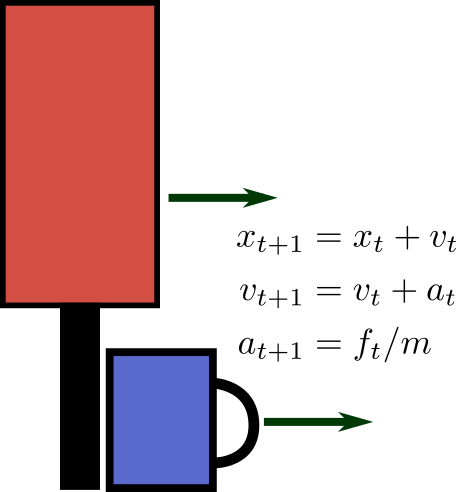
\includegraphics{tikz/lds}
    \caption{The graphical model for a linear dynamic system}
    \label{fig:graphical-model-lds}
\end{figure}

\subsection{Hierarchical clustering}
Hierarchical clustering is a structure learning problem
where the structure class is trees. Specifically,
given a dataset $\dataset$,
we are interested in rooted trees with $\numdata$ leaves
with each leaf corresponding to a data point.
Such a tree tree encodes relationships between data: 
if data points $a$ and $b$ are close in data space, we'd hope
the leaves corresponding to $a$ and $b$ appear closer
together in a tree that captures the data's structure.

Algorithms for hierarchical clustering can be broadly
divided into two categories: divisive and agglomerative.
Divisive, or top-down, clustering algorithms recover a tree by recursively
partitioning data until just leaves remain. Examples
include spectral clustering \citep{} and recursive $\k$-means.
Agglomerative, or bottom-up, clustering algorithms
initialize clusters as leaves, and recursively
merge clusters until a full binary tree is formed.
Pairs of clusters to merge are chosen according to
a heuristic, also called a linkage-criterion,
an example of which is single-linkage,
where clusters are merged according to the minimum
distance between data points in each cluster.

Hierarchical clustering can also be formalized as an optimization problem
by minimizing carefully constructed cost
function,
$C(\structure, \dataset)$,
as shown in \citet{Dasgupta2016}.
Treating this cost as the
energy in a Gibbs distribution,
we can also frame hierarchical clustering
as a probabilistic model
$\p(\dataset \given \tree) = \exp{-C(\tau, \dataset)/T}$ for some temperature $T$.
Recovering a hierarchical clustering of the
data is therefore a maximum likelihood problem:

\begin{align*}
    \tree^* = \argmax_{\tree} \exp{-C(\tau, \dataset)/T}
\end{align*}

\citet{Dasgupta2016} uses a greedy algorithm
to optimize this likelihood.
The graphical model for hierarchical clustering is pictured in \autoref{fig:graphical-model-hc}.

\begin{figure}[htp!]
    \centering
    \includegraphics{tikz/hc}
    \caption{Graphical model for hierarchical clustering}
    \label{fig:graphical-model-hc}
\end{figure}

\section{Bayesian structure learning}

Structure learning is an useful generalization
of several popular problems. However, it has some
drawbacks in its presented formulation.
Consider a dataset that has ambiguity in its
latent structure. For example, in \autoref{fig:ambiguous-structure}, we picture two examples of ambiguous latent structure. In a hierarchical clustering problem, if data are positioned in particular ways, we could organize the data
in several plausible ways. In one example, tare
three equally valid hierarchical clusterings (using binary trees), and in the second example, there are two
plausible clusterings. Structure learning as presented
cannot disambiguate between equally valid clusterings or indicate to a user that there exist alternative candidates.

\begin{figure*}[htp!]
    \centering
    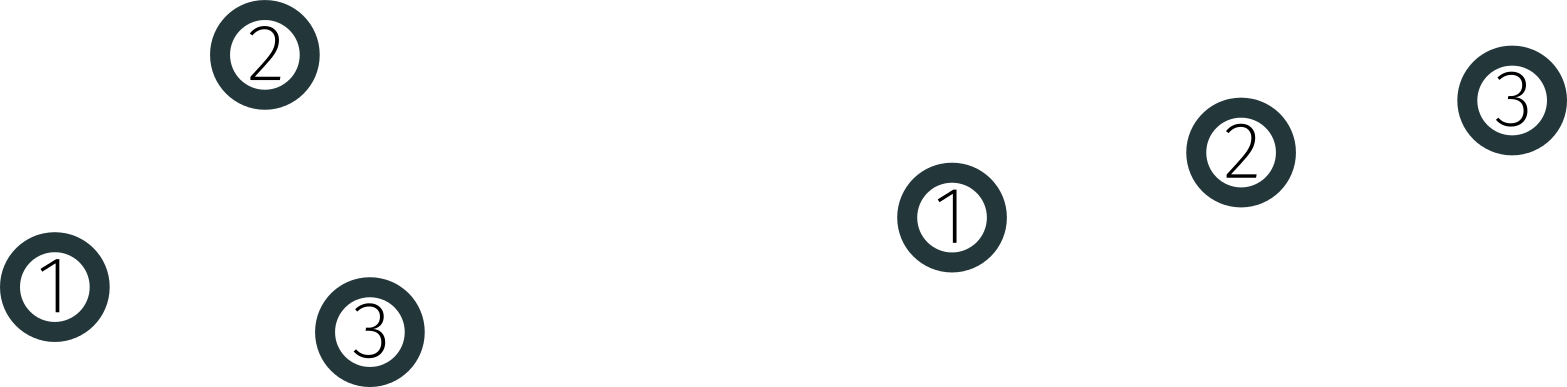
\includegraphics[width=0.8\textwidth]{img/structure/3-cluster-both}
    \caption{Examples of ambiguous hierarchical structure in data. The left set of points could plausibly be hierarchically clustered in three different ways, where any two points could be clustered before the other. The right set of points has two plausible hierarchical clusterings, where 1 and 2 could be clustered first, or 2 and 3 could be clustered first.}
    \label{fig:ambiguous-structure}
\end{figure*}

Bayesian structure learning puts a prior on the structure class $\p(\structure)$, and rather than
returning a candidate structure $\structure^*$,
it returns a posterior distribution over candidate
structures $\p(\structure \given \dataset)$. It generalizes 
vanilla structure learning, as $\p(\structure \given \dataset)$ could,
in principle,
be a delta distribution for a single candidate structure.
In practice, however, the Bayesian structure learning
formulation enables algorithms that capture
uncertainty and ambiguity in how data is organized.
In \autoref{fig:ambiguous-structure-probability},
we picture the same ambiguous hierarchical clusterings
along with the intuitively correct distribution over possible clusterings. 

\begin{figure*}[htp!]
    \centering
    \begin{subfigure}{\textwidth}
        \centering
        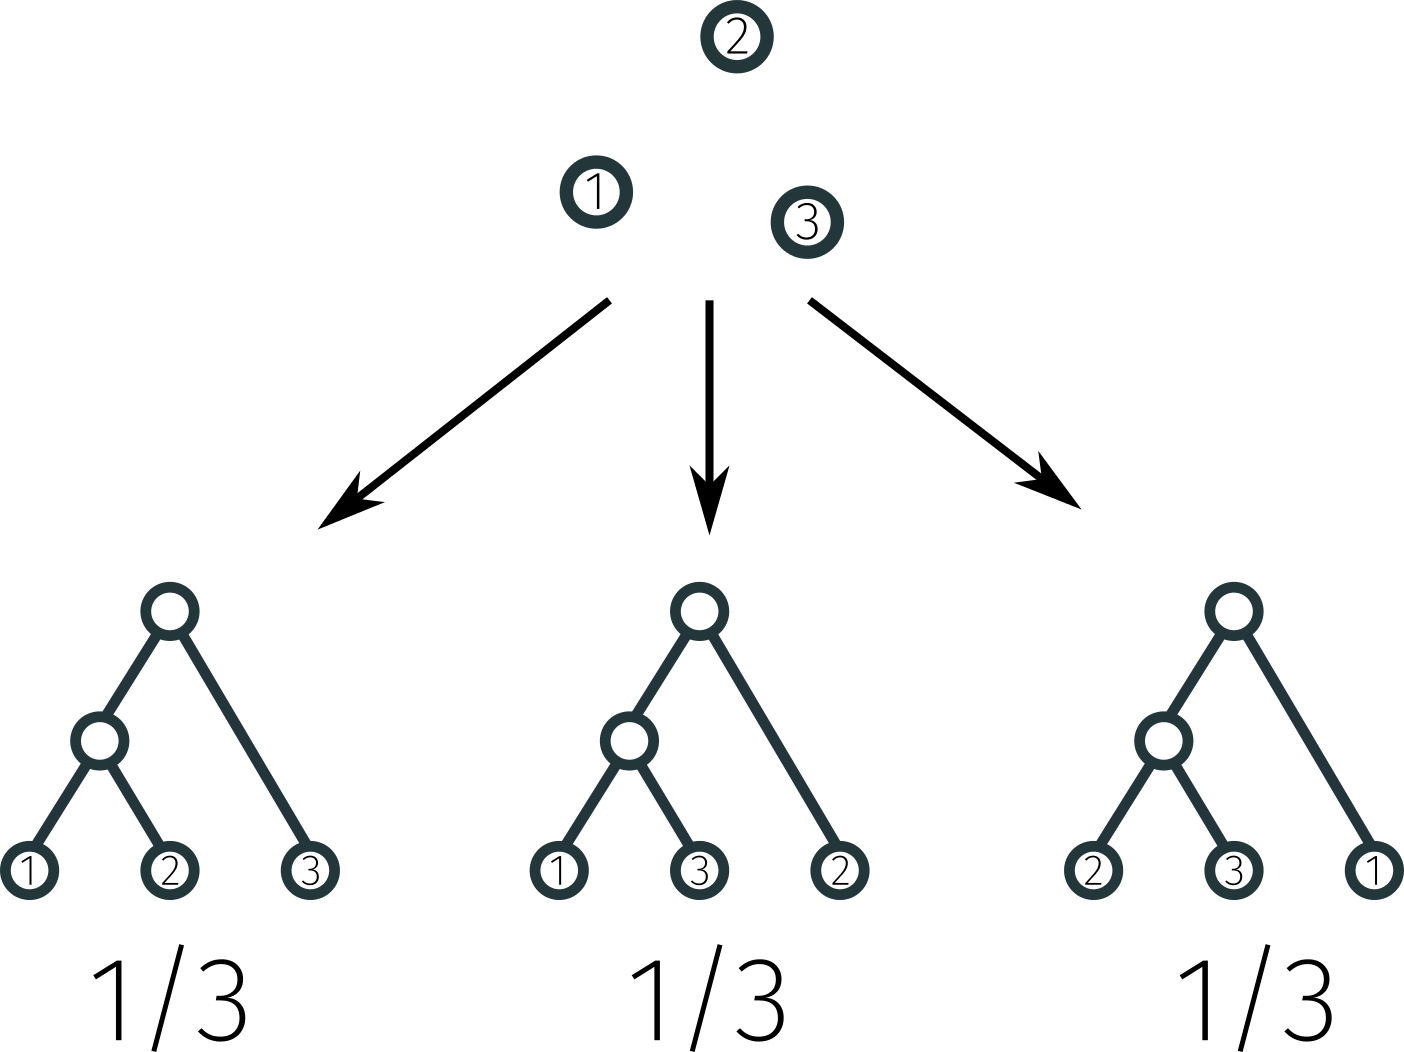
\includegraphics[width=0.7\textwidth]{img/structure/3-cluster-distribution}
        \caption{}
    \end{subfigure}
    \begin{subfigure}{\textwidth}
        \centering
        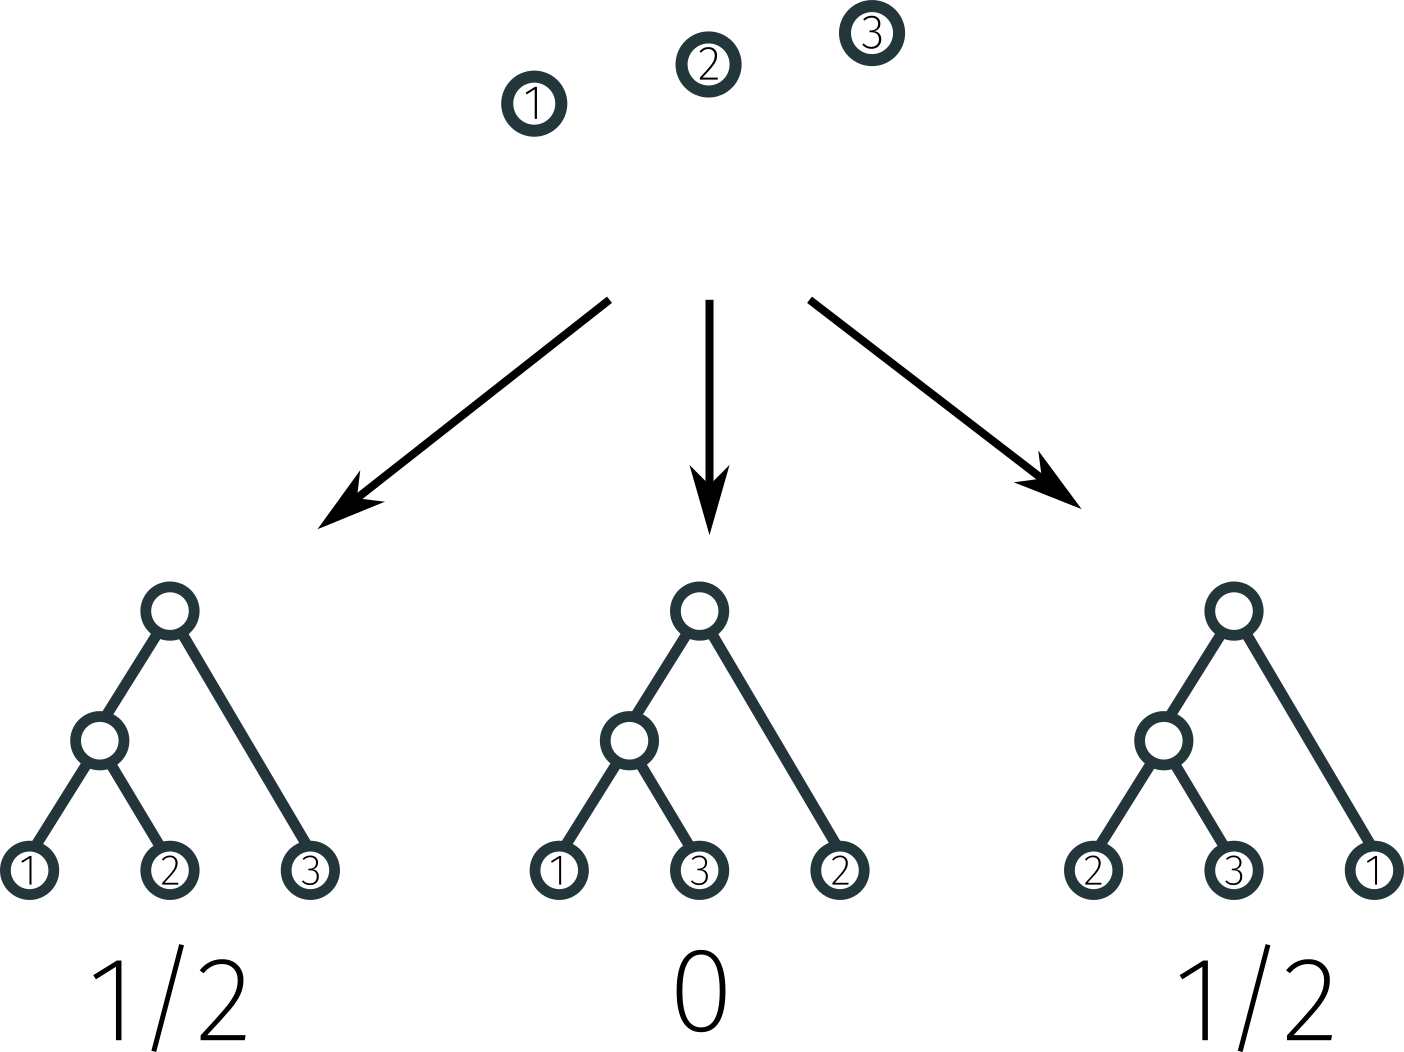
\includegraphics[width=0.7\textwidth]{img/structure/3-cluster-linear-distribution}
        \caption{}
    \end{subfigure}
    \caption{Examples of how Bayesian structure learning could resolve ambiguity in latent structure. In (a), all three possible clusterings are given equal probability and in (b), the two most likely clusterings split the probability.}
    \label{fig:ambiguous-structure-probability}
\end{figure*}

Bayesian structure learning can be formalized
as a latent variable model,
where we assume a prior over structures $\p(\structure)$,
and a likelihood model $p(\dataset \given \structure)$.
The goal is then to perform Bayesian
inference to obtain the posterior distribution $p(\structure \given \dataset)$. The simple graphical model for this generative process is pictured in \autoref{fig:graphical-model-bsl}.

\begin{figure}[htp!]
    \centering
    \includegraphics[]{tikz/lvm}
    \caption{The graphical model for Bayesian structure learning}
    \label{fig:graphical-model-bsl}
\end{figure}

The design space of Bayesian structure learning
amounts to first deciding a structure class (hierarchical clusterings, flat clusterings, linear dynamical systems, etc.) and additionally choosing a
particular prior distribution over the structures.
Although computing the posterior distribution $\p(\structure \given \dataset)$ amounts to Bayesian inference,
more often than not, this posterior distribution is analytically intractable and we must resort to
approximate inference. Thus, in practice, we must
also decide on an approximate inference algorithm (variational inference, MCMC, etc.).

\subsection{Bayesian linear dynamical system}

A Bayesian linear dynamical system (BLDS)
is an LDS with the addition of a prior
over the transition matrix and noise covariance. 
Although there are many choices of prior,
in this thesis, we use the matrix-Normal-inverse-Wishart (MNIW) prior, which is conjugate, details of which
are located in \autoref{sec:stats-mniw}.

The choice of this prior results in a generative model
\begin{align*}
    \dynmat, \dyncovar &\sim MNIW(\Psi, \dynmat_0, V, \nu) \\
    \state_{\t + 1} | \state_t, \dynmat, \dyncovar &\sim \N(\dynmat \state_t, \dyncovar)
\end{align*}
which is also visualized in \autoref{fig:graphical-model-blds}.

\begin{figure}[htp!]
    \centering
    \includegraphics[]{tikz/blds}
    \caption{The graphical model for a Bayesian linear dynamical system}
    \label{fig:graphical-model-blds}
\end{figure}

Because the MNIW prior is conjugate
with a linear dynamical system likelihood,
the posterior distribution $\p(\dynmat, \dyncovar \given \sequencen)$ is also MNIW
and can be computed in closed form.

Another structure class of interest is trees,
specifically hierarchical clusterings.
In the next chapter, we detail
how hierarchical clustering can be formalized 
in the Bayesian structure learning framework.